% Created 2022-03-12 Sat 10:34
% Intended LaTeX compiler: pdflatex
\documentclass[11pt]{article}
\usepackage[utf8]{inputenc}
\usepackage[T1]{fontenc}
\usepackage{graphicx}
\usepackage{grffile}
\usepackage{longtable}
\usepackage{wrapfig}
\usepackage{rotating}
\usepackage[normalem]{ulem}
\usepackage{amsmath}
\usepackage{textcomp}
\usepackage{amssymb}
\usepackage{capt-of}
\usepackage{hyperref}
\usepackage{braket}
\usepackage{relsize}
\usepackage{amsmath}
\newcommand{\kp}{\ket{\psi}}
\newcommand{\bp}{\bra{\psi}}
\newcommand{\tr}[1]{\textrm{tr}\left[{#1}\right]}
\newcommand{\U}{\mathcal{U}}
\author{Frank Lu}
\date{\today}
\title{}
\hypersetup{
 pdfauthor={Frank Lu},
 pdftitle={},
 pdfkeywords={},
 pdfsubject={},
 pdfcreator={Emacs 27.2 (Org mode 9.5)}, 
 pdflang={English}}
\begin{document}

\tableofcontents


% Boxed environment
\newsavebox{\mybox}
\newenvironment{Notes}
{\begin{lrbox}{\mybox}\begin{minipage}{\textwidth}}
{\end{minipage}\end{lrbox}\fbox{\usebox{\mybox}}\\}


% Theoretical results section
\newcommand{\nH}{n_H}
\newcommand{\nV}{n_V}
\newcommand{\NH}{N_H}
\newcommand{\NV}{N_V}

\newcommand{\ls}{l_1l_2 \dots l_{\nH}}
\newcommand{\ones}{1, 1, \dots, 1}
\newcommand{\ks}{k_1k_2 \dots k_{\nH}}

% Theoretical results section
\newcommand{\R}{\mathbb{R}}

\section{Burning questions}
\label{sec:org10ace28}
\begin{itemize}
\item Why use the Sigmoid function?
\begin{figure}[htbp]
\centering
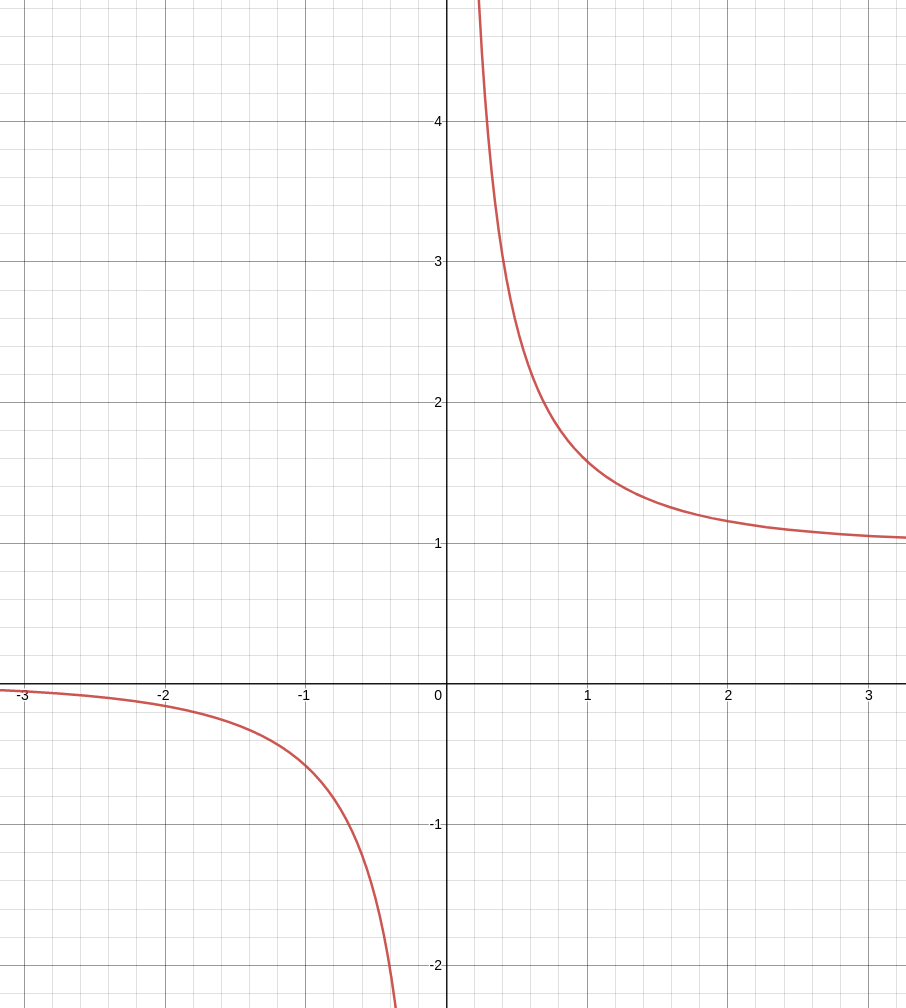
\includegraphics[scale=0.2]{/home/frank/shared/quantum/honours-thesis/rbm_learning/rbm_learning.org_20220305_105235_N9II2d.png}
\caption{The Logistic Sigmoid function}
\end{figure}

\item Multivariate calculus\ldots{}
\begin{center}
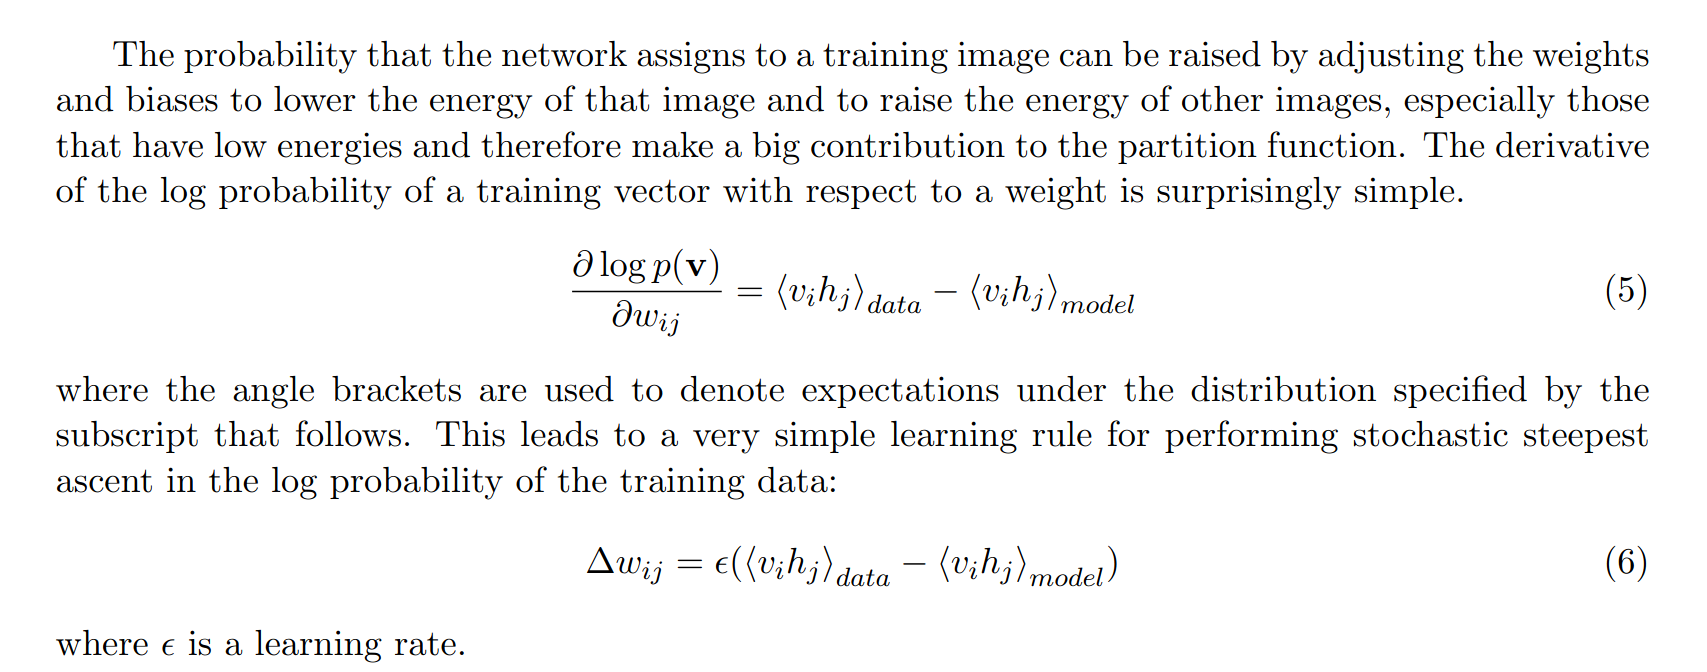
\includegraphics[scale=0.3]{/home/frank/shared/quantum/honours-thesis/rbm_learning/rbm_learning.org_20220305_105553_Ghq5ul.png}
\end{center}
\end{itemize}

\section{Very rough notes}
\label{sec:org9ef9dd7}
The family of gradient based leaning algorithms commonly used by RBMs is called \emph{Contrastive Divergence}.

\subsection{The RBM itself}
\label{sec:orgdc1bf97}
Assume your training set of binary images. Then, you can feed your image \(\mathbb{v}\) into the RBM.

\begin{center}
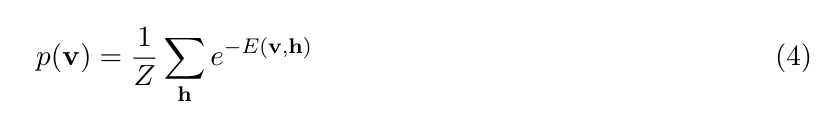
\includegraphics[width=.9\linewidth]{/home/frank/shared/quantum/honours-thesis/rbm_learning/rbm_learning.org_20220302_123159_1KYkb9.png}
\end{center}

Your \(\mathbf{h}\) vectors are binary vectors, and the sum is taken over all possible values of


\subsection{Contrastive Divergence}
\label{sec:org9b654ef}
Certain models result in an \emph{unnormalised probability distributions} (page 582, textbook), where the total probability is not 1.

\subsubsection{Partition Function}
\label{sec:orgb260372}
To normalise such a distribution \(\tilde{p}(\mathbf{x})\),

\begin{equation}
p(\mathbf{x}) = \frac{1}{Z} \tilde{p}(\mathbf{x})
\end{equation}

And, \(Z\) which is called the \emph{partition function} is defined as follows for continuous variables.

\begin{equation}
Z = \int \tilde{p}(\mathbf{x}) d\mathbf{x}
\end{equation}

Or, for discrete variables

\begin{equation}
Z = \sum_{\mathbf{x}} \tilde{p}(\mathbf{x})
\end{equation}

Note that the argument to \(Z\) is often omitted in the literature.

Usually, it is intractable to compute \(Z\) directly, so an approximation is used.

\begin{Notes}
!Gibbs distribution! -- distribution of product of clique potentials.
\end{Notes}

\section{Machine learning notes}
\label{sec:org00cf8e4}
Here, I will briefly give the background for machine learning in the context of RBMs.

Machine learning algorithms are used when it is difficult to directly write an algorithm to do some task. For example, computer vision, or speech recognition.


Mathematically, we want some function \(f\) given some input to produce an output, but \(f\) cannot be readily defined so we opt for a (not necessarily probablistic) but 'good enough' model. In this case, it is sensible to choose a family of functions (?) \(f ( x ; \theta )\) parameterised by \(\theta\) as our model. In a sense, a good model will have a good choice of \(f\), in that \(f\) is able to approximate the distribution of our outputs, and a good choice of \(\theta\).

We will start with supervised learning, where we have a set \(X = \{x_1, x_2, \dots, x_k \}\) of \(k\) inputs and \(Y = \{y_1, y_2, \dots, y_k\}\) outputs. Our goal is to find \(f : X \to \hat{Y}\), where \(\hat{Y} = \{ \hat{y}_1, \hat{y}_2, \dots, \hat{y}_k\}\) and for all \(i\), \(f(x_i) = \(\hat{y}_i\). The hats on the \(Y\)s is to show that this just an approximation for actual \(y\) values. Of course, a good model will be one such that for all \(i\), \(\hat{y}_i \approx y_i\).


\emph{Linear regression} is a good example of a machine learning algorithm.

\subsection{Finding a good parameterisation}
\label{sec:org13b8959}
What is a good choice of \(\theta\)? It only makes sense to ask this question if we can measure the performance of a particular choice of \(\theta\). To this end, let \(C(f, \theta)\) be the cost function that produces a scalar output. So now, the best choice of \(\theta\) is one that optimises \(C\).

A simple and commonly used cost function is the mean squared error, \(C(Y, \hat{Y}) = \sum_i (y_i - \hat{y}_i)^2\)



\subsection{Mathematical fundamentals}
\label{sec:org33f1fba}
\emph{From scratch} spends a lot of time talking about calculating gradients to functions.

Suppose, \(f : A \to A\), \(g : (A, A) \to A\). Then, given the map \(Z(x, y) = (f \circ g) (x, y)\), we want to find out how the gradient of the output with respect to the input. More precisely, \(\frac{dZ}{dx}\) and \(\frac{dZ}{dy}\).
(This is done using the chain rule).

The backward pass is precisely the act of finding gradients with respect to the input variables.




\section{Understanding: Learning for undirected models}
\label{sec:org48920c9}
\subsection{Partition Functions}
\label{sec:org864bc16}
\subsection{Maximum likelihood}
\label{sec:orgc2c3d90}
``Negative phase is very hard''. So naive algorithm isn't used.

\subsubsection{Contrastive Divergence}
\label{sec:org76255e1}
\end{document}
